\documentclass{beamer}
\usepackage{geometry}
\usepackage[english]{babel}
\usepackage[utf8]{inputenc}
\usepackage{amsmath}
\usepackage{amsfonts}
\usepackage{amssymb}
\usepackage{tikz}
\usetikzlibrary{quotes, angles}
\usepackage{graphicx}

\usepackage{multicol}
%\usepackage{pgfplots}
%\pgfplotsset{width=10cm,compat=1.9}
%\usepackage{pgfplotstable}

\usepackage{fancyhdr}
\pagestyle{fancy}
\setlength{\headheight}{12pt}%doesn't seem to fix warning
\fancyhf{}

%\rhead{\small{24 February 2020}}
\lhead{\small{BECA / Dr. Huson / Unit 9: Congruence \& similarity transformations}}

\renewcommand{\headrulewidth}{0pt}

\title{Mathematics Class Slides}
\subtitle{Bronx Early College Academy}
\author{Chris Huson}
\date{9 March 2020}

\begin{document}
\frame{\titlepage}
\section[Outline]{}
\frame{\tableofcontents}

\section{10.1 Tangent applications, Monday 9 March} 
\frame
{
  \frametitle{GQ: How do we apply trig functions to solve problems?}
  \framesubtitle{CCSS: HSG.CO.B6-8 Understand congruence in terms of rigid motions \hfill \alert{10.1 Monday  9 March}}

  \begin{block}{Do Now: Transformations}
  \begin{itemize}
    \item Rigid motions: translation, reflection, rotation
    \item Corresponding angles and lengths
    \item Symmetry in terms of transformations ``onto'' itself
    \item Using the properties of rigid motions in explanations
  \end{itemize}
  \end{block}
  Lesson: Point-slope linear equation format \\
  Tangent review, segment dilation\\*[5pt]
  Homework: Trig Deltamath practice
}

\section{10.2 Exam review, Gradescope intro; Tuesday 10 March} 
\frame
{
  \frametitle{GQ: How do we learn from exam results using Gradescope?}
  \framesubtitle{CCSS: HSG.CO.B6-8 Understand congruence in terms of rigid motions \hfill \alert{10.2 Tuesday 10 March}}

  \begin{block}{Do Now: Algebra mastery practice on Deltamath}
    \begin{itemize}
      \item Circle equations (use Casio calculator)
      \item Linear equations of parallel \& perpendicular lines
    \end{itemize}
    \end{block}
    Lesson: Setting up and using Gradescope exam scoring system \\
    Test corrections due at the end of class (classwork credit)\\*[5pt]
    Homework: Complete DoNow Deltamath problems (due 10PM)
}

\section{10.3 Tangent situations, ladders, Wednesday 11 March} 
\frame
{
  \frametitle{GQ: How do we solve a triangle given an angle measure?}
  \framesubtitle{CCSS: HSG.CO.B6-8 Understand congruence in terms of rigid motions \hfill \alert{10.3 Wednesday 11 March}}

  \begin{block}{Do Now: Rigid motions, translation, reflection, rotation}
    \begin{itemize}
      \item Perpendicular and parallel slopes
      \item Circle equations
      \item Point-slope form of linear equations
      \item Reflection vs rotation
    \end{itemize}
    \end{block}
    Lesson: Diagraming ladder problems, using the tangent function \\
    Homework: Complete transformations practice handout
}

\section{10.4 Tangent situations, ladders, Thursday 12 March} 
  \frame
  {
    \frametitle{GQ: How do we solve a triangle given an angle measure?}
    \framesubtitle{CCSS: HSG.CO.B6-8 Understand congruence in terms of rigid motions \hfill \alert{10.4 Thursday 12 March}}

    \begin{block}{Do Now: Rigid motions, translation, reflection, rotation}
      \begin{itemize}
        \item Tangent calculations
        \item Compositions of transformations
        \item Reflection vs rotation
      \end{itemize}
      \end{block}
      Lesson: Diagraming ladder problems, using the tangent function \\
      Homework: Complete transformations practice handout
  }

\section{10.5 Deltamath trig practice, Friday 13 March} 
\frame
{
  \frametitle{GQ: How do we solve a triangle given an angle measure?}
  \framesubtitle{CCSS: HSG.CO.B6-8 Understand congruence in terms of rigid motions \hfill \alert{10.5 Friday 13 March}}

  \begin{block}{Do Now: Right triangle trigonometry}
    \begin{multicols}{2}
    \begin{itemize}
      \item Find $AB$
      \item Find $\tan A$
      \item Find $\tan B$
      \item Find $m\angle A$
    \end{itemize}
    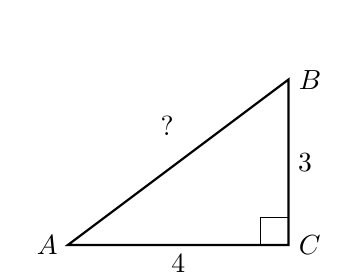
\begin{tikzpicture}[scale=0.7]
      \draw [thick]
      (0,0)node[left]{$A$}--
      (4,0)node[ right]{$C$}--
      (4,3)node[right]{$B$}--cycle;
      \draw (4,0)++(-0.5,0)--++(0,0.5)--+(0.5,0);
      \node at (2,0)[below]{$4$};
      \node at (4,1.5)[right]{$3$};
      \node at (1.8,1.8)[above]{$?$};
    \end{tikzpicture}
  \end{multicols}
    \end{block}
    Classwork: Deltamath trigonometry practice \\
    Homework: Complete trig practice on Deltamath
}

\end{document}

